\subsection{替换算法对 Cache 命中率的影响}

当 Cache 发生 Miss 且目标 Set 已满时，需要根据替换算法选择一个 Cache Line 换出。不同替换算法对程序局部性的利用程度不同，因此可能会对 Cache 命中率产生影响。本组实验对比 FIFO 和 LRU 两种替换策略在相同 Cache 配置下的表现。

\subsubsection{实验设计}

本组实验采用矩阵规模为 $N=128$ 时生成的 trace.log 作为输入，固定 Cache 块大小为 64B，映射方式为 4 路组相联，分别测试 FIFO 和 LRU 两种替换算法下的 Cache 命中率。

实验固定参数如下：

\begin{itemize}
    \item 矩阵规模：$N=128$；
    \item Cache 块大小：64B；
    \item 映射方式：4 路组相联；
    \item 输入文件：$N=128$ 时由 NEMU 生成的 trace.log。
\end{itemize}

变化参数为替换算法：

\begin{itemize}
    \item FIFO：先进先出替换算法；
    \item LRU：最近最少使用替换算法。
\end{itemize}

\subsubsection{实验结果}

\begin{table}[H]
\centering
\caption{FIFO 与 LRU 替换算法对命中率的影响}
\begin{tabular}{c|c|c|c}
\hline
Cache 大小 & 替换算法 & 命中率(\%) & Miss 数 \\
\hline
16KB & FIFO & 49.76 &2136344 \\
16KB & LRU  & 49.75 & 2136615 \\
32KB & FIFO & 49.77 & 2135968 \\
32KB & LRU  & 49.76 & 2136208 \\
64KB & FIFO & 97.27 & 116087 \\
64KB & LRU  & 97.26 & 116568 \\
128KB & FIFO & 99.85 & 6174 \\
128KB & LRU  & 99.83 & 7200 \\
\hline
\end{tabular}
\end{table}
实验数据绘制如下图:
\begin{figure}[H]
    \centering
    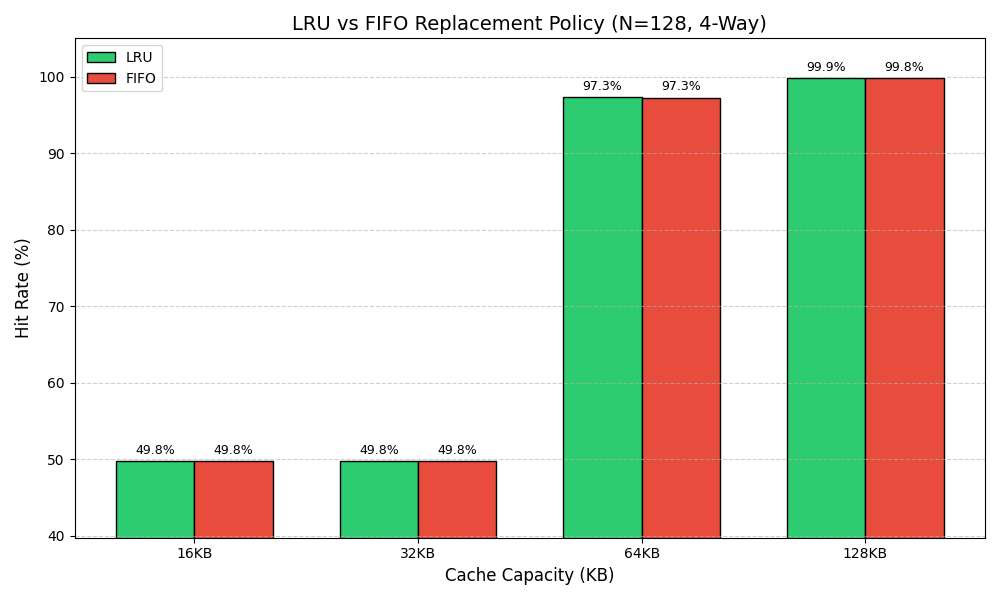
\includegraphics[width = 1\textwidth]{figure/replacement_policy_impact.png}
    \caption{替换策略对Cache命中率的影响}
\end{figure}

\subsubsection{实验现象与分析}

从实验结果可以看出，在本组矩阵乘法 trace 下，FIFO 和 LRU 两种替换算法的命中率差异很小，整体表现非常接近。具体而言，在 16KB、32KB、64KB 和 128KB 四种 Cache 容量下，FIFO 的命中率分别为 49.76\%、49.77\%、97.27\% 和 99.85\%；LRU 的命中率分别为 49.75\%、49.76\%、97.26\% 和 99.83\%。从数值上看，FIFO 在本实验中反而略高于 LRU，但差距均较小。

在 16KB 和 32KB 的低容量阶段，两种算法的命中率都维持在约 49.7\%。这说明此时主要瓶颈并不是替换算法选择，而是 Cache 容量不足。由于矩阵规模为 $N=128$ 时三个矩阵总大小达到 192KB，而 16KB 和 32KB 的 Cache 远不能容纳主要工作集，因此大量 Miss 属于容量缺失。在这种情况下，即使使用 LRU，也难以通过保留“最近访问的数据”显著改善命中率。

当 Cache 容量增加到 64KB 和 128KB 时，两种算法的命中率都明显提高，说明容量增加消除了大量容量缺失。此时 FIFO 和 LRU 的差距仍然很小，说明该矩阵乘法访问序列在当前配置下对替换策略并不十分敏感。换言之，影响命中率的主要因素是 Cache 容量是否能够覆盖足够大的活跃工作集，而不是 FIFO 与 LRU 之间的细微差别。

从理论上看，LRU 更符合时间局部性原理，因为它倾向于保留最近被访问过的数据块；FIFO 实现更简单，但不关心数据近期是否被访问。然而，本实验数据说明，理论上更复杂的 LRU 并不一定在所有访存序列下都优于 FIFO。对于本实验中的矩阵乘法 trace，FIFO 和 LRU 的结果几乎相同，并且 FIFO 略优。

\subsubsection{实验总结}

通过 FIFO 和 LRU 的对比可以看出，替换算法对命中率的影响依赖于具体访存序列和 Cache 容量。在本实验中，FIFO 与 LRU 的命中率差距很小，且 FIFO 在各组容量下均略高于 LRU，因此不能简单得出“LRU 一定优于 FIFO”的结论。

更准确地说，LRU 是一种符合时间局部性思想的通用替换策略，在许多存在明显重复访问的程序中可能表现较好；但当程序的主要 Miss 来源是容量不足，或者访问模式使得替换策略难以发挥作用时，LRU 的优势会被削弱。对于本实验的矩阵乘法 trace，Cache 容量对命中率的影响明显大于替换算法本身。